\documentclass[tikz,border=10pt]{standalone}
\begin{document}
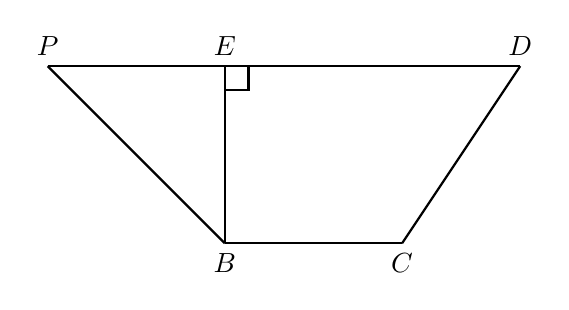
\begin{tikzpicture}[thick, scale=1.5]
    % 1. 定义坐标点
    % 假设 B 点为原点 (0,0)，根据比例设定各点位置
    \coordinate (B) at (0,0);
    \coordinate (C) at (1.5,0);
    \coordinate (E) at (0,1.5);
    \coordinate (P) at (-1.5,1.5);
    \coordinate (D) at (2.5,1.5);

    % 2. 绘制图形轮廓
    \draw (P) -- (D);        % 顶部的水平线 PD
    \draw (P) -- (B);        % 左侧斜线 PB
    \draw (B) -- (C);        % 中间底部水平线 BC
    \draw (C) -- (D);        % 右侧斜线 CD
    \draw (E) -- (B);        % 垂直辅助线 EB

    % 3. 标注顶点标签
    \node[above] at (P) {$P$};
    \node[above] at (E) {$E$};
    \node[above] at (D) {$D$};
    \node[below] at (B) {$B$};
    \node[below] at (C) {$C$};

    % 4. 可选：标注直角
    % 在 E 点处增加直角标记
    \draw (0, 1.3) -- (0.2, 1.3) -- (0.2, 1.5);

\end{tikzpicture}
\end{document}